% ============================================================
% Capítulo V — Polarización rotatoria. Dispersión
% Traducción de "Théorie mathématique de la lumière" (1889), cap. V
% Original: §§121-143, páginas impresas 176-216 (PDF 192-232)
% ============================================================
\chapter{Polarización rotatoria. Dispersión}
\label{cap:polarizacion-dispersion}

\noindent\textbf{121.} Para hallar las ecuaciones
\begin{equation}
-\rho\frac{d^2\xi}{dt^2}=\sum\frac{d}{dx}\cdot\frac{dW_2}{d\xi'_x},\qquad
-\rho\frac{d^2\eta}{dt^2}=\sum\frac{d}{dx}\cdot\frac{dW_2}{d\eta'_x},\qquad
-\rho\frac{d^2\zeta}{dt^2}=\sum\frac{d}{dx}\cdot\frac{dW_2}{d\zeta'_x}
\tag{1}
\end{equation}
del movimiento de una molécula en un medio elástico (§32), admitimos (§14)
que las cantidades $D x,Dy,Dz$ eran del orden del radio de actividad
molecular, por lo que podíamos, en las expresiones de $D\xi,D\eta,D\zeta$,
despreciar los términos que contienen $Dx^2,Dy^2,Dz^2$. De ello resultaba
que $D\xi,D\eta,D\zeta$ eran funciones lineales de las nueve derivadas
parciales de $\xi,\eta,\zeta$ respecto de las variables $x,y,z$, y que
$W_2$ era una función homogénea y de segundo orden respecto de esas nueve
derivadas.

Buscamos luego (§41) en qué se convertían las ecuaciones (1) en el caso de
los medios isótropos, y vimos (§42) que el movimiento de las moléculas en
ese medio se propagaba con una velocidad constante
$V=\sqrt{-2\mu/\rho}$.

Ahora bien, la experiencia demuestra que, cuando la luz atraviesa un medio
isótropo distinto del éter en el vacío, su velocidad depende de su longitud
de onda $\lambda$; nos vemos, pues, conducidos a pensar que la hipótesis
del §14, que no está justificada por ninguna consideración teórica, debe
rechazarse cuando consideramos la propagación de la luz en un medio
ponderable. Si abandonamos esta hipótesis, las cantidades $D\xi,D\eta,D\zeta$
contendrán las derivadas de los diversos órdenes de $\xi,\eta,\zeta$
respecto de $x,y,z$, y, por consiguiente, la función $W_2$, que es
homogénea y de segundo grado (§13) en $D\xi,D\eta,D\zeta$, será homogénea y
de segundo grado respecto de las derivadas parciales de los diversos
órdenes de $\xi,\eta,\zeta$. Vamos a mostrar que las ecuaciones del
movimiento de una molécula, tomando para $W_2$ una función de esta clase,
explican el fenómeno de la dispersión y el de la polarización rotatoria.

\noindent\textbf{122.} Designando por $U$ la función de fuerzas relativa a
las fuerzas exteriores e interiores que se ejercen sobre las moléculas de
un volumen $R$ limitado por una superficie $S$ (figura~\ref{fig:cap5-1}),
hallamos (§27), por la aplicación del principio de d'Alembert y del
principio de las velocidades virtuales, la ecuación
\begin{equation}
\delta U - \int \rho\,d\tau\left(\frac{d^2\xi}{dt^2}\delta\xi
+\frac{d^2\eta}{dt^2}\delta\eta+\frac{d^2\zeta}{dt^2}\delta\zeta\right)=0,
\tag{2}
\end{equation}
que debe satisfacerse cualesquiera que sean $\delta\xi,\delta\eta,\delta\zeta$.

\begin{figure}[h]
\centering
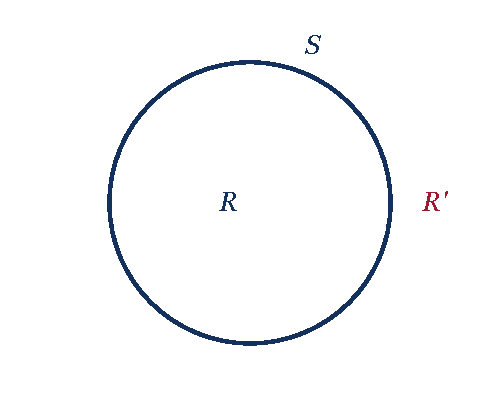
\includegraphics[width=0.45\textwidth]{figuras/pdf/cap05-fig1.pdf}
\caption{Superficie $S$ que limita un volumen $R$, con el medio exterior
$R'$.}
\label{fig:cap5-1}
\end{figure}

La parte de la función $U$ que corresponde a las fuerzas interiores es
$\int \delta W\,d\tau$, y la relativa a las fuerzas exteriores que se
ejercen sobre la superficie de separación $S$ es
$\int(\mathrm P_x\delta\xi+\mathrm P_y\delta\eta+\mathrm P_z\delta\zeta)\,d\omega$,
designando $\mathrm P_x,\mathrm P_y,\mathrm P_z$ las componentes, según los
tres ejes, de la presión que se ejerce sobre el elemento de superficie
$d\omega$. Sustituyendo $\delta U$ por la suma de estas dos cantidades, la
ecuación (2) se convierte en
\[
\int(\mathrm P_x\delta\xi+\mathrm P_y\delta\eta+\mathrm P_z\delta\zeta)\,d\omega
+\int\delta W\,d\tau
-\int\rho\,d\tau\left(\frac{d^2\xi}{dt^2}\delta\xi+\frac{d^2\eta}{dt^2}\delta\eta
+\frac{d^2\zeta}{dt^2}\delta\zeta\right)=0.
\]
Como esta ecuación debe satisfacerse cualesquiera que sean
$\delta\xi,\delta\eta,\delta\zeta$, podemos, en particular, suponer
$\delta\eta=\delta\zeta=0$, y tenemos la igualdad
\begin{equation}
\int \mathrm P_x\delta\xi\,d\omega + \int\delta W\,d\tau
-\int\frac{d^2\xi}{dt^2}\delta\xi\,\rho\,d\tau=0,
\tag{3}
\end{equation}
que deberá cumplirse cualquiera que sea $\delta\xi$.

\noindent\textbf{123.} Se trata de transformar el segundo término de esta
igualdad. La función $W$ es, en general, una función de las derivadas
parciales de los diversos órdenes de $\xi,\eta,\zeta$. En un desplazamiento
virtual cualquiera dado al sistema, cada una de estas derivadas varía,
pero, en el caso en que se tiene, como hemos supuesto, $\delta\eta=\delta\zeta=0$,
solo cambian de valor las derivadas parciales de $\xi$. Por consiguiente,
el incremento $\delta W$ de la función $W$ dependerá únicamente de los
incrementos de las distintas derivadas parciales de $\xi$. Con el fin de
simplificar los cálculos, admitiremos que las únicas derivadas parciales de
$\xi$ que entran en $W$ son $d\xi/dx$ y $d^2\xi/dx^2$, derivadas que
podremos representar sin ambigüedad por $\xi'$ y $\xi''$. Tenemos
entonces,
\[
\delta W = \frac{dW}{d\xi'}\delta\xi' + \frac{dW}{d\xi''}\delta\xi'',
\]
y, por consiguiente,
\[
\int\delta W\,d\tau = \int\frac{dW}{d\xi'}\delta\xi'\,d\tau
+\int\frac{dW}{d\xi''}\delta\xi''\,d\tau.
\]
Se sabe, y recordamos esta propiedad en el §30, que se tiene
\begin{equation}
\int\frac{dW}{d\xi'}\delta\xi'\,d\tau
=\int\alpha\frac{dW}{d\xi'}\delta\xi\,d\omega
-\int\delta\xi\,\frac{d}{dx}\cdot\frac{dW}{d\xi'}\,d\tau,
\tag{4}
\end{equation}
y
\[
\int\frac{dW}{d\xi''}\delta\xi''\,d\tau
=\int\alpha\frac{dW}{d\xi''}\delta\xi'\,d\omega
-\int\delta\xi'\,\frac{d}{dx}\cdot\frac{dW}{d\xi''}\,d\tau.
\]
Esta última igualdad se convierte, al hacer sufrir a la segunda integral
del segundo miembro una transformación análoga, en
\begin{equation}
\int\frac{dW}{d\xi''}\delta\xi''\,d\tau
=\int\alpha\frac{dW}{d\xi''}\delta\xi'\,d\omega
-\int\alpha\delta\xi\,\frac{d}{dx}\cdot\frac{dW}{d\xi''}\,d\omega
+\int\delta\xi\,\frac{d^2}{dx^2}\cdot\frac{dW}{d\xi''}\,d\tau.
\tag{5}
\end{equation}
Sumando los segundos miembros de las igualdades (4) y (5), y sustituyendo
en (3) la segunda integral por esta suma, obtenemos una igualdad que
contiene integrales extendidas a la superficie $S$ e integrales extendidas
al volumen $R$. Representando la suma de las integrales dobles por $I$, la
ecuación (3) se convierte en
\[
I - \int\left(\frac{d}{dx}\cdot\frac{dW}{d\xi'}
-\frac{d^2}{dx^2}\cdot\frac{dW}{d\xi''}+\rho\frac{d^2\xi}{dt^2}\right)\delta\xi\,d\tau=0,
\]
y, como debe satisfacerse cualquiera que sea $\delta\xi$, el elemento
diferencial colocado bajo el signo de integración extendido al volumen debe
ser nulo. Tendremos, pues,
\[
\rho\frac{d^2\xi}{dt^2} = -\frac{d}{dx}\cdot\frac{dW}{d\xi'}
+\frac{d^2}{dx^2}\cdot\frac{dW}{d\xi''}.
\]
Esta ecuación se convierte, designando por $W_1$ el término de primer
grado y por $W_2$ el término de segundo grado en el desarrollo de $W$
según las potencias crecientes de $D\xi,D\eta,D\zeta$, en
\[
\rho\frac{d^2\xi}{dt^2} = -\frac{d}{dx}\cdot\frac{dW_1}{d\xi'}
+\frac{d^2}{dx^2}\cdot\frac{dW_1}{d\xi''}
-\frac{d}{dx}\cdot\frac{dW_2}{d\xi'}+\frac{d^2}{dx^2}\cdot\frac{dW_2}{d\xi''}.
\]
Pero, siendo $D\xi,D\eta,D\zeta$ de primer grado (§14) respecto de las
derivadas parciales de $\xi,\eta,\zeta$, lo mismo ocurrirá con $W_1$; las
derivadas de esta función respecto de $\xi'$ y $\xi''$ serán constantes, y
la ecuación anterior se reduce a
\[
\rho\frac{d^2\xi}{dt^2} = -\frac{d}{dx}\cdot\frac{dW_2}{d\xi'}
+\frac{d^2}{dx^2}\cdot\frac{dW_2}{d\xi''}.
\]
Esta es la primera de las ecuaciones del movimiento de una molécula; las
otras dos se obtendrían de la misma manera.

En cuanto a la suma de integrales que hemos designado por $I$, nos daría el
valor de las presiones que se ejercen sobre la superficie $S$. No
buscaremos esas presiones.

\section{Ecuaciones del movimiento}

\noindent\textbf{124. Ecuaciones del movimiento.} — Nos vemos así
conducidos a la siguiente regla. Las ecuaciones del movimiento se escribirán
\[
\rho\frac{d^2\xi}{dt^2}=\mathrm P,\qquad
\rho\frac{d^2\eta}{dt^2}=\mathrm Q,\qquad
\rho\frac{d^2\zeta}{dt^2}=\mathrm R,
\]
siendo $\mathrm P,\mathrm Q,\mathrm R$ polinomios lineales respecto de las
derivadas de los diversos órdenes de $\xi,\eta,\zeta$, y formados de la
manera siguiente:

Para formar $\mathrm P$, se diferenciará $W_2$ respecto de cada una de las
derivadas parciales de $\xi$ que figuran en ella. Se diferenciará la
derivada de $W_2$ así obtenida, respecto de $x$, $y$ y $z$, de la misma
manera que se hizo con la derivada parcial de $\xi$ que figura en ella. Por
ejemplo, se diferenciará
\[
\frac{dW_2}{d\xi'_x}\ \text{una vez respecto de }x,\qquad
\frac{dW_2}{d\xi''_{xx}}\ \text{dos veces respecto de }x,\qquad
\frac{dW_2}{d\xi''_{xy}}\ \text{una vez respecto de }x\text{ y una respecto de }y,\ \text{etc.}
\]
Se sumarán luego todas las derivadas así obtenidas, tras haber afectado del
signo $+$ las derivadas de orden par y del signo $-$ las derivadas de orden
impar. Tendremos, pues,
\[
\mathrm P = -\frac{d}{dx}\frac{dW_2}{d\xi'_x}-\frac{d}{dy}\frac{dW_2}{d\xi'_y}
-\frac{d}{dz}\frac{dW_2}{d\xi'_z}
+\frac{d^2}{dx^2}\frac{dW_2}{d\xi''_{xx}}+\cdots
+\frac{d^2}{dxdy}\frac{dW_2}{d\xi''_{xy}}+\cdots
-\frac{d^3}{dx^3}\frac{dW_2}{d\xi'''_{xxx}}-\cdots
\]

Se formaría el polinomio $\mathrm Q$ de la misma manera, diferenciando
$W_2$ respecto de las derivadas parciales de $\eta$.

En algunos casos particulares, la expresión del polinomio $\mathrm P$ se
simplifica. Así, si el medio elástico es isótropo, las derivadas de orden
impar no entran en $\mathrm P$. En efecto, en tal medio, las ecuaciones del
movimiento no deben cambiar cuando se cambian a la vez los signos de
$x,y,z,\xi,\eta,\zeta$. Ahora bien, al hacer este cambio, $d^2\xi/dt^2$
cambia de signo; por consiguiente, los distintos términos de $\mathrm P$
deben cambiar también de signo. Esto ocurre para todas las derivadas de
orden par respecto de $x,y,z$, pero las derivadas de orden impar, como
$d^3\xi/dx^3$, $d^3\xi/(dx^2dy)$, conservan el mismo valor puesto que sus
numeradores y sus denominadores cambian de signo al mismo tiempo. Estas
derivadas no podrán, pues, entrar en la expresión del polinomio $\mathrm P$
relativo a un medio isótropo.

Cuando el medio elástico tiene un centro de simetría, las ecuaciones del
movimiento no deben cambiar cuando se cambian los signos de
$x,y,z,\xi,\eta,\zeta$. También en este caso, el polinomio $\mathrm P$ no
deberá contener más que derivadas de orden par.

\section{Polarización rotatoria del cuarzo}

\noindent\textbf{125. Polarización rotatoria del cuarzo.} — Puesto que el cuarzo cristaliza bajo una forma
hemiédrica del sistema romboédrico, los cristales de cuarzo no poseen
centro de simetría.

Si admitimos que la distribución del éter luminoso en un cuerpo ponderable
es idéntica a la de las moléculas materiales que constituyen el cuerpo, el
éter contenido en el cuarzo será un medio elástico desprovisto de centro de
simetría.

Por consiguiente, el polinomio $\mathrm P$ que entra en las ecuaciones del
movimiento de las moléculas de éter que propagan la luz en el cuarzo podrá
contener derivadas parciales de $\xi,\eta,\zeta$ de orden impar. Vamos a
mostrar, colocándonos en condiciones particulares para evitar cálculos
demasiado largos, que la presencia de las derivadas de tercer orden basta
para dar cuenta de los fenómenos de polarización rotatoria que presenta el
cuarzo.

Consideremos una onda cuyo plano sea perpendicular al eje del cristal.
Tomando para plano de las $xy$ un plano paralelo al de la onda, los
desplazamientos $\xi,\eta,\zeta$ de las moléculas de éter no dependerán más
que de $z$ y del tiempo $t$, y, por consiguiente, las derivadas parciales
de los diversos órdenes de $\xi,\eta,\zeta$ respecto de $x$ y de $y$ serán
nulas. Además, como las vibraciones son transversales, la condición de
transversalidad, $\Theta=0$, exige que se tenga idénticamente $\zeta'_z=0$.
Por consiguiente, $W_2$ será una función homogénea y de segundo grado de
las derivadas parciales de primer orden $\xi'_z,\eta'_z$ y de las derivadas
parciales de órdenes superiores de $\xi,\eta,\zeta$ respecto de $z$.
Designemos por $W_2^1$ el conjunto de los términos de $W_2$ que son
homogéneos respecto de las derivadas parciales de primer orden y, para
simplificar\footnote{Véase más adelante el capítulo relativo a la doble
refracción en los medios hemiédricos, donde volvemos sobre esta cuestión
con más detalle.}, supongamos que los demás términos de $W_2$ sean nulos,
con excepción del siguiente:
\[
a\,\frac{d\eta}{dz}\,\frac{d^2\xi}{dz^2}.
\]

Aplicando la regla que dimos (§124) para la formación de los segundos
miembros de las ecuaciones del movimiento, obtenemos para esas ecuaciones:
\[
\rho\frac{d^2\xi}{dt^2}=-\sum\frac{d}{dx}\frac{dW_2^1}{d\xi'_x}+a\frac{d^3\eta}{dz^3},
\qquad
\rho\frac{d^2\eta}{dt^2}=-\sum\frac{d}{dx}\frac{dW_2^1}{d\eta'_x}-a\frac{d^3\xi}{dz^3}.
\]

Los términos de los segundos miembros provenientes de $W_2^1$ serán las
derivadas parciales de segundo orden de $\xi,\eta,\zeta$, multiplicadas por
un coeficiente constante. Admitamos que, en la primera ecuación, estos
términos se reducen a $d^2\xi/dz^2$ y que, en la segunda, se reducen a
$d^2\eta/dz^2$; tendremos entonces, para las ecuaciones del movimiento:
\begin{equation}
\rho\frac{d^2\xi}{dt^2}=\frac{d^2\xi}{dz^2}+a\frac{d^3\eta}{dz^3},
\tag{1}
\end{equation}
\begin{equation}
\rho\frac{d^2\eta}{dt^2}=\frac{d^2\eta}{dz^2}-a\frac{d^3\xi}{dz^3}.
\tag{2}
\end{equation}

Busquemos satisfacer estas ecuaciones\footnote{A
partir de aquí, el original reinicia con frecuencia su numeración local de
ecuaciones varias veces dentro de este mismo capítulo (como ya ocurrió en
los capítulos II y IV); conservamos fielmente la numeración de Poincaré en
cada caso, sin forzar una numeración continua.} poniendo
\[
\xi=\mathrm Ae^{\frac{2i\pi}{\lambda}(z-Vt)},\qquad
\eta=\mathrm Be^{\frac{2i\pi}{\lambda}(z-Vt)}.
\]
Las derivadas parciales de $\xi$ y $\eta$ que entran en las ecuaciones del
movimiento tendrán por valor
\[
\frac{d^2\xi}{dt^2}=\mathrm A\left(\frac{2i\pi}{\lambda}\right)^2\mathrm V^2
e^{\frac{2i\pi}{\lambda}(z-Vt)},\qquad
\frac{d^2\eta}{dt^2}=\mathrm B\left(\frac{2i\pi}{\lambda}\right)^2\mathrm V^2
e^{\frac{2i\pi}{\lambda}(z-Vt)},
\]
\[
\frac{d^2\xi}{dz^2}=\mathrm A\left(\frac{2i\pi}{\lambda}\right)^2
e^{\frac{2i\pi}{\lambda}(z-Vt)},\qquad
\frac{d^2\eta}{dz^2}=\mathrm B\left(\frac{2i\pi}{\lambda}\right)^2
e^{\frac{2i\pi}{\lambda}(z-Vt)}.
\]
Llevando estos valores a las ecuaciones (1) y (2), y suprimiendo los
factores comunes a ambos miembros, obtenemos,
\begin{equation}
\mathrm A(\rho\mathrm V^2-1)=a\mathrm B\,\frac{2i\pi}{\lambda},
\tag{3}
\end{equation}
\begin{equation}
\mathrm B(\rho\mathrm V^2-1)=-a\mathrm A\,\frac{2i\pi}{\lambda}.
\tag{4}
\end{equation}
Dividiendo estas ecuaciones miembro a miembro tendremos,
\[
\frac{\mathrm A}{\mathrm B}=-\frac{\mathrm B}{\mathrm A};
\]
igualdad que puede ponerse en la forma
\[
\mathrm A^2=-\mathrm B^2,
\]
de donde
\[
\mathrm A=\pm \mathrm Bi.
\]
Podremos, pues, satisfacer las ecuaciones del movimiento tomando para
$\xi$ y $\eta$ las partes reales de
\[
\xi_1=\mathrm Bi\,e^{\frac{2i\pi}{\lambda}(z-Vt)},\qquad
\eta_1=\mathrm Be^{\frac{2i\pi}{\lambda}(z-Vt)},
\]
o de
\[
\xi_2=-\mathrm Bi\,e^{\frac{2i\pi}{\lambda}(z-Vt)},\qquad
\eta_2=\mathrm Be^{\frac{2i\pi}{\lambda}(z-Vt)}.
\]
El primer sistema de soluciones nos da, para los desplazamientos de la
molécula en el plano $z=0$, expresiones de la forma
\[
\xi_1=r\cos(\alpha t+\varphi),\qquad \eta_1=r\sin(\alpha t+\varphi).
\]
El segundo sistema nos da, para los desplazamientos en el mismo plano,
\[
\xi_2=-r\cos(\alpha t+\varphi),\qquad \eta_2=r\sin(\alpha t+\varphi).
\]
Para obtener la curva descrita por la molécula en el plano de las $x,y$,
basta eliminar $t$ entre los valores de $\xi$ y $\eta$. Tendremos, sumando
los cuadrados de $\xi_1$ y $\eta_1$ y los cuadrados de $\xi_2$ y $\eta_2$,
las dos ecuaciones
\[
\xi_1^2+\eta_1^2=r^2,\qquad \xi_2^2+\eta_2^2=r^2.
\]
Estas ecuaciones muestran que, en ambos casos, la trayectoria de la
molécula será un círculo; pero, siendo los valores de $\xi_1$ y de $\xi_2$
de signos contrarios, estos dos círculos se recorrerán en sentidos
contrarios. Por consiguiente, una onda plana que se propaga en un cristal
de cuarzo puede considerarse como desdoblándose en dos ondas planas
polarizadas circularmente, una en un sentido, la otra en sentido contrario.
Nos basta ahora mostrar que la propagación de estas ondas se hace con
velocidades distintas para que quede explicada la polarización rotatoria
del cuarzo.

Para obtener estas velocidades, hagamos sucesivamente, en una de las
fórmulas (3) o (4), $\mathrm A=\mathrm Bi$ y $\mathrm A=-\mathrm Bi$;
obtendremos:\footnote{En rigor, $\mathrm A=\mathrm Bi$ da
$\rho\mathrm V^2-1=+a\,2\pi/\lambda$ y $\mathrm A=-\mathrm Bi$ da
$\rho\mathrm V^2-1=-a\,2\pi/\lambda$, es decir, el orden inverso al que
indica el original. La inversión solo intercambia los papeles de
$\mathrm V_1$ y $\mathrm V_2$ y no afecta en nada a lo que sigue;
conservamos el orden de Poincaré.}
\[
\rho\mathrm V^2-1=-a\,\frac{2\pi}{\lambda},\qquad
\rho\mathrm V^2-1=a\,\frac{2\pi}{\lambda};
\]
de donde sacamos, para los cuadrados de las velocidades $\mathrm V_1$ y
$\mathrm V_2$ de las dos ondas polarizadas,
\begin{equation}
\mathrm V_1^2=\frac{1}{\rho}-\frac{a}{\rho}\,\frac{2\pi}{\lambda},
\tag{5}
\end{equation}
\begin{equation}
\mathrm V_2^2=\frac{1}{\rho}+\frac{a}{\rho}\,\frac{2\pi}{\lambda}.
\tag{6}
\end{equation}
Como $a$ no es nulo, tenemos para $\mathrm V_1$ y $\mathrm V_2$ valores
distintos; por consiguiente, en la propagación en el cuarzo de una onda
plana polarizada, el plano de polarización de esta onda debe girar.

\noindent\textbf{126.} De los valores que acabamos de hallar para las
velocidades de propagación de las ondas polarizadas circularmente, es fácil
deducir la ley de Biot sobre el poder rotatorio del cuarzo, es decir,
mostrar que este poder rotatorio varía en razón inversa del cuadrado de la
longitud de onda.

\begin{enunciado}{Ley de Biot}
El poder rotatorio del cuarzo varía en razón inversa del cuadrado de la
longitud de onda.
\end{enunciado}

Designando por $e$ el espesor de la lámina de cuarzo atravesada por los
rayos luminosos, la diferencia de marcha de estos rayos, a la salida de la
lámina, será
\[
\frac{e}{\mathrm V_1}\mathrm V-\frac{e}{\mathrm V_2}\mathrm V,
\]
siendo $\mathrm V$ la velocidad de propagación en el vacío.

Ahora bien, se sabe que la rotación del plano de polarización es igual a
$360^{\circ}$ cuando la diferencia de marcha es igual a la longitud de onda. Por
consiguiente, el espesor de una lámina de cuarzo que hace girar $360^{\circ}$ el
plano de polarización viene dado por la fórmula
\[
\mathrm V\left(\frac{e}{\mathrm V_1}-\frac{e}{\mathrm V_2}\right)=\lambda,
\]
de donde
\[
e=\frac{\lambda}{\mathrm V}\,\frac{\mathrm V_1\mathrm V_2}{\mathrm V_2-\mathrm V_1}.
\]
Restando una de otra las igualdades (5) y (6), obtenemos
\[
\mathrm V_2^2-\mathrm V_1^2=\frac{4\pi}{\lambda}\frac{a}{\rho},
\]
de donde sacamos
\[
\frac{1}{\mathrm V_2-\mathrm V_1}=\frac{(\mathrm V_1+\mathrm V_2)\lambda}{4\pi}\frac{\rho}{a}.
\]
La expresión de $e$ se convierte, al sustituir en ella este valor de
$1/(\mathrm V_2-\mathrm V_1)$, en
\[
e=\frac{\lambda^2\mathrm V_1\mathrm V_2(\mathrm V_1+\mathrm V_2)}{4\pi\mathrm V}\frac{\rho}{a}.
\]
Como el valor de $a$ es muy pequeño, podemos, en los valores de
$\mathrm V_1^2$ y de $\mathrm V_2^2$, despreciar el segundo término frente
al primero, y se tiene $\mathrm V_1=\mathrm V_2=1/\sqrt{\rho}$.
Sustituyendo $\mathrm V_1$ y $\mathrm V_2$ por este valor en la expresión
anterior, obtenemos
\[
e=\frac{\lambda^2}{2\pi a\mathrm V\sqrt\rho}.
\]
El espesor capaz de hacer girar $360^{\circ}$ el plano de polarización es, pues,
proporcional a $\lambda^2$; de ello se deduce inmediatamente que la
rotación producida por una lámina cuyo espesor es igual a la unidad varía
en razón inversa del cuadrado de la longitud de onda.

Las experiencias muy precisas han mostrado que esta ley no se verifica
rigurosamente; este resultado no debe sorprendernos, pues los cálculos que
hemos hecho no son sino aproximados.

\section{Polarización rotatoria de los cristales y las disoluciones}

\noindent\textbf{127. Polarización rotatoria de los cristales y las
disoluciones.} — Existe cierto número de sustancias cristalizadas
que presentan, aunque en grado menor que el cuarzo, la propiedad de hacer
girar el plano de polarización de la luz. Como, hasta ahora, todos los
cristales para los que se ha constatado esta propiedad son cristales
hemiédricos, se les puede aplicar la explicación que hemos dado del poder
rotatorio del cuarzo. Pero se conoce un gran número de sustancias orgánicas
cuyas disoluciones gozan del poder rotatorio, y, en ese caso, la
explicación del fenómeno se vuelve más difícil: los líquidos se comportan
en general como cuerpos isótropos. No se ha hallado por lo demás una
explicación satisfactoria, y nos vemos obligados a admitir que esas
sustancias orgánicas destruyen la isotropía de los líquidos, y que sus
disoluciones, que tienen una infinidad de ejes de simetría, no tienen, sin
embargo, centro de simetría.

\section{Explicación de la dispersión}

\noindent\textbf{128. Explicación de la dispersión.} — No nos ocuparemos por el momento más que de cuerpos
isótropos o de cuerpos con centro de simetría. En este último caso tomaremos
el centro de simetría como origen de las coordenadas. Los segundos miembros
de las ecuaciones del movimiento no contendrán entonces más que derivadas
parciales de orden par de $\xi,\eta,\zeta$ respecto de $x,y,z$.

Consideremos una onda plana que se propaga en tal medio, y tomemos para
plano de las $xy$ un plano paralelo al plano de la onda. Los desplazamientos
$\xi,\eta,\zeta$, no dependiendo más que de $z$ y de $t$, las únicas
derivadas parciales de estas cantidades que entrarán en los segundos
miembros de las ecuaciones del movimiento serán las derivadas parciales de
orden par respecto de $z$. Admitiendo la transversalidad de las vibraciones,
la condición $\Theta=0$ nos da, para el valor de $\zeta'_z$, la identidad
$\zeta'_z=0$; por consiguiente, las derivadas parciales de $\zeta$ son
idénticamente nulas, y los segundos miembros de las ecuaciones del
movimiento no pueden contener más que las cantidades
\[
\frac{d^2\xi}{dz^2},\frac{d^4\xi}{dz^4},\frac{d^6\xi}{dz^6},\ldots,
\frac{d^2\eta}{dz^2},\frac{d^4\eta}{dz^4},\frac{d^6\eta}{dz^6},\ldots.
\]
Tomemos la primera de las ecuaciones,
\[
\rho\frac{d^2\xi}{dt^2}=\mathrm P.
\]
Esta ecuación no debe cambiar por la sustitución de $-y$ a $y$ y de $-\eta$
a $\eta$, en el caso de los cuerpos isótropos, o en el caso de los cuerpos
que posean un centro de simetría cuando se toma ese punto como origen de
los ejes. Ahora bien, el primer miembro de la ecuación no cambiando de
signo por esta sustitución, las derivadas parciales de $\eta$,
$d^2\eta/dz^2,d^4\eta/dz^4,\ldots$, cuyo signo cambiaría, no deben entrar
en el polinomio $\mathrm P$. Por consiguiente, el segundo miembro de la
ecuación no puede contener más que las derivadas de $\xi$. Limitándonos a
las derivadas de orden inferior al octavo, esta ecuación se convierte en
\[
\rho\frac{d^2\xi}{dt^2}=a\frac{d^2\xi}{dz^2}+b\frac{d^4\xi}{dz^4}
+c\frac{d^6\xi}{dz^6}.
\]
Un razonamiento idéntico nos mostraría que la segunda ecuación del
movimiento de las moléculas de una onda plana que se propaga en un medio
isótropo o en un medio con centro de simetría se reduce a
\[
\rho\frac{d^2\eta}{dt^2}=a\frac{d^2\eta}{dz^2}+b\frac{d^4\eta}{dz^4}
+c\frac{d^6\eta}{dz^6}.
\]
Si buscamos satisfacer estas ecuaciones mediante expresiones de $\xi$ y
$\eta$ de la forma siguiente
\[
\xi=\mathrm Ae^{\frac{2i\pi}{\lambda}(z-Vt)},\qquad
\eta=\mathrm Be^{\frac{2i\pi}{\lambda}(z-Vt)},
\]
obtendremos dos ecuaciones de condición que contienen la velocidad $V$ de
propagación. Para mostrar que $V$ depende de la longitud de onda $\lambda$
de la radiación, nos basta tomar una de estas ecuaciones. Calculando las
derivadas parciales de $\xi$ y sustituyendo los valores hallados en la
primera de las ecuaciones del movimiento, obtendremos, tras dividir por el
factor común a ambos miembros,
\[
\left(\frac{2i\pi}{\lambda}\right)^2\mathrm Ae^{\frac{2i\pi}{\lambda}(z-Vt)},
\]
la relación siguiente:
\[
\rho\mathrm V^2=a+b\left(\frac{2i\pi}{\lambda}\right)^2
+c\left(\frac{2i\pi}{\lambda}\right)^4
\]
o
\[
\rho\mathrm V^2=a-\frac{4\pi^2 b}{\lambda^2}+\frac{16\pi^4c}{\lambda^4}.
\]

Siendo el índice de refracción $n$ proporcional al inverso de la
velocidad, tendremos una cantidad proporcional a $n$ tomando la potencia
$-\tfrac12$ del segundo miembro de esta última relación: como los términos
en $1/\lambda^2$ y $1/\lambda^4$ son correcciones pequeñas frente al
término constante $a$, basta desarrollar
$\bigl(a-4\pi^2b/\lambda^2+16\pi^4c/\lambda^4\bigr)^{-1/2}$ por la fórmula
del binomio y detenerse en los términos en $1/\lambda^4$, sin olvidar que el
cuadrado del término en $1/\lambda^2$ contribuye también a este orden; se
halla así
\[
a^{-1/2}\left[1+\frac{2\pi^2b}{a}\,\frac{1}{\lambda^2}
+\left(\frac{6\pi^4b^2}{a^2}-\frac{8\pi^4c}{a}\right)\frac{1}{\lambda^4}
+\cdots\right],
\]
que reproduce, con nuevas constantes, la misma forma en $1/\lambda^2$ y
$1/\lambda^4$. Por consiguiente, podemos escribir:

\begin{enunciado}{Fórmula de Cauchy}
\[
n=\mathrm A_0+\frac{\mathrm B_0}{\lambda^2}+\frac{\mathrm C_0}{\lambda^4}.
\]
\end{enunciado}

\noindent Esta fórmula, hallada por Cauchy, nos muestra que el índice de
refracción varía con la longitud de onda y que, por consiguiente, las
diversas radiaciones de una luz heterogénea serán desigualmente desviadas.
La comparación de los valores de $n$ calculados por esta fórmula con los
valores hallados por la experiencia ha mostrado que hay una concordancia
muy satisfactoria para todas las radiaciones luminosas. Los resultados de
la experiencia quedan ya suficientemente bien representados cuando no se
toman más que los dos primeros términos de la fórmula.

\section{Teorías diversas de la dispersión}

\noindent\textbf{129. Teorías diversas de la dispersión.} — La teoría de la dispersión que acabamos de exponer
supone que, cuando la luz atraviesa un medio ponderable, las cantidades del
orden del cuadrado del radio de actividad molecular no son despreciables.
Puesto que podíamos despreciar esas cantidades cuando, en los capítulos
precedentes, no nos ocupábamos más que de la propagación de la luz en el
vacío y en que solo considerábamos la acción del éter sobre sí mismo,
debemos concluir que la materia actúa sobre las moléculas de éter, y que el
radio de actividad de las moléculas materiales es incomparablemente mayor
que el de las moléculas de éter. Esta acción de la materia sobre el éter
ya había sido admitida por Fresnel, quien suponía que el éter contenido en
los medios ponderables tenía una densidad constante pero mayor que en el
vacío. Más tarde, Cauchy, con el fin de explicar la dispersión, admitió
implícitamente que las moléculas materiales son arrastradas por las
moléculas de éter y que vibran con la misma amplitud. Aunque esta última
hipótesis pueda parecer poco verosímil, no hay que apresurarse a
rechazarla; así es como un cuerpo que flota en la superficie de un líquido
participa, por arrastre, de los movimientos que se imprimen al líquido. En
todo caso, es esta hipótesis la que condujo a Cauchy al análisis del
n.\textsuperscript{o}~128, cuyo acuerdo con la experiencia hemos visto.

Después de Cauchy, Briot retomó el estudio de la dispersión. En una
primera teoría, admitió el arrastre de la materia por el éter, pero supuso
que las amplitudes de las vibraciones de las moléculas materiales eran
incomparablemente más pequeñas que las amplitudes de las moléculas de
éter. Resultaba de esta hipótesis que, en los cálculos, se podían
considerar las moléculas materiales como fijas respecto de las moléculas
de éter. En estas condiciones, los segundos miembros de las ecuaciones del
movimiento de una molécula de éter contenían, además de las derivadas
segundas de $\xi,\eta,\zeta$, esas mismas cantidades. La velocidad de
propagación del movimiento vibratorio dependía entonces de la longitud de
onda, y el índice de refracción venía dado por una fórmula de la forma
\[
n=\mathrm A+\mathrm B\lambda^2.
\]
Pero, hallándose esta fórmula en contradicción con los resultados de la
experiencia, Briot se vio llevado a rechazar esta teoría y propuso otra
que vamos a exponer.

\section{Teoría de Briot}

\noindent\textbf{130. Teoría de Briot.}\footnote{Hemos conservado el
nombre de teoría de Briot a la explicación que vamos a desarrollar, porque
Briot fue el primero que intentó fundar una teoría completa de la
dispersión sobre la hipótesis de la periodicidad del éter. Pero el modo de
exposición que seguiremos difiere por completo del de Briot y se acerca
bastante más a las ideas de M. Sarrau.} — En esta teoría, Briot, al
considerar los medios ponderables como formados de moléculas materiales
separadas unas de otras, admite que la densidad del éter contenido en ese
medio es tanto mayor cuanto más próxima está la molécula de éter de una
molécula material. Resulta de ello que esta densidad $\rho$ es una función
de las coordenadas de la molécula considerada.

Hasta aquí, hemos supuesto constante la densidad del éter, y en el §33
mostramos que, en esa hipótesis y despreciando las cantidades del orden
del cuadrado del radio de actividad molecular, el movimiento de una
molécula de éter venía dado por tres ecuaciones, de las cuales la primera
era\footnote{El original impreso dice aquí $\mu\Delta\xi$; es una errata
evidente por $2\mu\Delta\xi$, como muestran la ecuación del §33 y la forma
$-2\mu(\Delta\xi-d\Theta/dx)$ que se deduce a continuación.}
\[
-\rho\frac{d^2\xi}{dt^2}=2\mu\Delta\xi+2\nu\frac{d\Theta}{dx}.
\]
Admitiendo (§46) que se tiene $\nu=-\mu$, esta ecuación se reduce a
\[
\rho\frac{d^2\xi}{dt^2}=-2\mu\left(\Delta\xi-\frac{d\Theta}{dx}\right).
\]
El coeficiente $-2\mu$ es positivo, pues la velocidad de propagación de
las vibraciones transversales es real y hemos visto que esta velocidad
viene dada por la fórmula
\[
\mathrm V^2=\frac{-2\mu}{\rho}.
\]
Por consiguiente, podremos, mediante una elección conveniente de la unidad
de fuerza, hacer de modo que se tenga $-2\mu=+1$. La primera de las
ecuaciones del movimiento se convierte entonces en
\begin{equation}
\rho\frac{d^2\xi}{dt^2}=\Delta\xi-\frac{d\Theta}{dx}.
\tag{1}
\end{equation}
Se sabe que es fácil hallar una solución de esta ecuación cuando $\rho$ es
una cantidad constante, pero la complicación del problema se vería
singularmente aumentada si $\rho$ dependiera de las coordenadas de la
molécula vibrante. Para conciliar la hipótesis fundamental de la densidad
variable del éter con las exigencias del cálculo, admitiremos además que
el radio de actividad molecular del éter es muy pequeño, y que, en el
interior de una esfera de radio igual al radio de actividad molecular, la
densidad puede considerarse como constante. Resultará de ello que en esa
esfera el movimiento de una molécula viene dado por tres ecuaciones
análogas a la ecuación (1). Trataremos de seguir, sin detenernos en el modo
de exposición de Briot, cómo estas hipótesis pueden dar cuenta de la
dispersión en los cuerpos cristalizados y en los cuerpos amorfos.

\section{Caso de los cuerpos cristalizados}

\noindent\textbf{131. Caso de los cuerpos cristalizados.} — Se sabe que,
apoyándose en consideraciones cuya idea se debe a Bravais, se pueden
considerar los cuerpos cristalizados como formados por moléculas
materiales que ocupan los vértices de paralelepípedos iguales y
yuxtapuestos. Las caras de estos paralelepípedos formarán tres sistemas de
planos que podemos representar mediante las ecuaciones
\begin{equation}
ax+by+cz=dm,
\tag{1}
\end{equation}
\begin{equation}
a'x+b'y+c'z=d'm',
\tag{2}
\end{equation}
\begin{equation}
a''x+b''y+c''z=d''m'',
\tag{3}
\end{equation}
en las cuales $m,m',m''$ serán enteros que varían de $-\infty$ a
$+\infty$. Los valores de $x,y,z$ que satisfacen estas tres ecuaciones
serán las coordenadas de un vértice de un paralelepípedo. Tomemos uno de
estos puntos $\mathrm P$ y démosle a sus coordenadas incrementos
$\alpha,\beta,\gamma$ que satisfagan las ecuaciones siguientes
\begin{equation}
a\alpha+b\beta+c\gamma=d,
\tag{4}
\end{equation}
\begin{equation}
a'\alpha+b'\beta+c'\gamma=0,
\tag{5}
\end{equation}
\begin{equation}
a''\alpha+b''\beta+c''\gamma=0.
\tag{6}
\end{equation}
Las dos últimas ecuaciones muestran que el punto $\mathrm P'$ de
coordenadas $x+\alpha,y+\beta,z+\gamma$ está situado en los planos de los
sistemas (2) y (3) que pasan por el punto $x,y,z$. De la ecuación (4) se
sigue que las coordenadas del punto $\mathrm P'$ satisfacen la ecuación
\[
a(x+\alpha)+b(y+\beta)+c(z+\gamma)=d(m+1).
\]
Por consiguiente, el punto $\mathrm P'$ se encontrará en el plano del
sistema (1) que es el más próximo al plano de ese mismo sistema que pasa
por el punto $\mathrm P$. Los puntos $\mathrm P$ y $\mathrm P'$ forman, por
tanto, los extremos de una arista de un paralelepípedo, y, en
consecuencia, $\alpha,\beta,\gamma$ son las proyecciones de esta arista
sobre los tres ejes.

Se vería de la misma manera que las proyecciones $\alpha',\beta',\gamma'$
y $\alpha'',\beta'',\gamma''$ de las otras dos aristas de los
paralelepípedos vienen dadas por ecuaciones que se deducen fácilmente de
las ecuaciones (4), (5) y (6).

\noindent\textbf{132.} Establecidos estos preliminares, volvamos a la
teoría de Briot. Sean $x,y,z$ las coordenadas de un punto cualquiera del
espacio; la densidad del éter en ese punto es una cierta función de
$x,y,z$ que representaremos por $\mathrm F(x,y,z)$. Si damos a las
coordenadas los incrementos $\alpha,\beta,\gamma$, obtendremos un nuevo
punto que estará evidentemente situado respecto de los vértices de un
cierto paralelepípedo contiguo como el punto $x,y,z$ se encuentra situado
respecto de los vértices de uno de los paralelepípedos. Puesto que la
posición de estos dos puntos respecto de las moléculas materiales es la
misma, la densidad del éter en esos puntos debe tener el mismo valor.
Tendremos, pues,
\[
\rho=\mathrm F(x,y,z)=\mathrm F(x+\alpha,y+\beta,z+\gamma);
\]
es decir, que la densidad es una función periódica de las coordenadas.

Dando a las coordenadas $x,y,z$ los incrementos iguales a las proyecciones
de las otras dos aristas de los paralelepípedos, obtendremos dos nuevos
puntos en los que el éter tiene la misma densidad; por consiguiente,
tenemos
\[
\rho=\mathrm F(x,y,z)=\mathrm F(x+\alpha',y+\beta',z+\gamma')
=\mathrm F(x+\alpha'',y+\beta'',z+\gamma'').
\]
La densidad $\rho$ del éter en un medio cristalizado es, pues, una función
triplemente periódica de las coordenadas.

\noindent\textbf{133.} Consideremos una onda plana que se propaga en un
medio cristalizado y tomemos para plano de las $xy$ un plano paralelo al
de la onda. Sabemos que $\xi,\eta,\zeta$ no dependen entonces más que de
$z$ y de $t$, y que resulta de la condición de transversalidad que
$\zeta$ es idénticamente nulo. Estando la densidad supuesta constante en
el interior de una esfera de radio igual al radio de actividad molecular,
$\rho$ será independiente de los desplazamientos $\xi,\eta,\zeta$ y será
únicamente función de las coordenadas de la posición de equilibrio de la
molécula considerada. Como solo queremos, por el momento, poner de
manifiesto la influencia de la periodicidad y mostrar que basta para
explicar la dispersión, supondremos, para simplificar, que $\rho$ es una
función periódica \emph{de $z$ únicamente}, y que, por consiguiente, puede
desarrollarse en serie trigonométrica. Pondremos
\[
\rho=\mathrm L_0+\mathrm L_1\cos z+\cdots+\mathrm M_1\sin z
+\mathrm M_2\sin 2z+\cdots.
\]

Demostremos que la condición necesaria y suficiente para que una función
periódica $\varphi$ sea la derivada de una función periódica $\psi$ es que
el valor medio de $\varphi$ sea nulo. Para ello desarrollemos $\varphi$ en
serie trigonométrica; tendremos
\[
\varphi=a_0+a_1\cos z+a_2\cos 2z+\cdots+b_1\sin z+b_2\sin 2z+\cdots.
\]
Si damos a $z$ todos los valores posibles, las funciones seno y coseno que
entran en este desarrollo tomarán una infinidad de valores comprendidos
entre $+1$ y $-1$; el valor medio de esas funciones será, pues, nulo, y,
por consiguiente, el valor medio de $\varphi$ se reduce a $a_0$. La
integral indefinida de $\varphi$ será
\[
\psi=c+a_0z+a_1\sin z+a_2\sin 2z+\cdots-b_1\cos z-b_2\cos 2z-\cdots.
\]
Cuando el valor medio $a_0$ de $\varphi$ es nulo, esta integral es una
función periódica de $z$. La condición enunciada es, pues, necesaria; es
evidente que es suficiente. Nos serviremos de esta propiedad de las
funciones periódicas en lo que sigue.

\noindent\textbf{134.} Tomemos ahora las ecuaciones del movimiento. Por la
transversalidad de las vibraciones, la ecuación (1) del §130 se convierte,
en el caso de una onda plana paralela al plano de las $xy$, en
\[
\rho\frac{d^2\xi}{dt^2}=\frac{d^2\xi}{dz^2}.
\]
Tratemos de satisfacer esta ecuación poniendo
\[
\xi=e^{i\mu t+\int v\,dz},
\]
siendo $\mu$ igual a $-2\pi/\lambda$ y siendo $v$ una función periódica de
$z$. Tendremos, para las derivadas primeras y segundas de $\xi$ respecto de
$t$ y de $z$:
\[
\frac{d\xi}{dt}=i\mu\xi,\qquad \frac{d\xi}{dz}=v\xi,\qquad
\frac{d^2\xi}{dt^2}=-\mu^2\xi,\qquad
\frac{d^2\xi}{dz^2}=v^2\xi+\xi\frac{dv}{dz}.
\]
Llevando estos valores de las derivadas segundas a la ecuación del
movimiento, tenemos\footnote{El original impreso dice $dv/dx$; es una
errata evidente por $dv/dz$, pues $v$ solo depende de $z$, como confirma el
desarrollo del §135.}
\begin{equation}
\frac{dv}{dz}+v^2+\rho\mu^2=0,
\tag{1}
\end{equation}
ecuación diferencial que da el valor de $v$ en función de $z$ y de $\mu$.
Observemos que, a consecuencia de la unidad de longitud adoptada, la
cantidad $\mu$ es muy pequeña. En efecto, esta unidad, elegida de modo que
el periodo de la función periódica $\rho$ sea finito, es comparable con
las dimensiones del paralelepípedo elemental, es decir, muy pequeña
respecto de $\lambda$; por consiguiente, $\lambda$ se expresará mediante un
número muy grande, y $\mu$, que es su inverso, será un número muy pequeño.
Resulta de ello que, si desarrollamos $v$ según las potencias crecientes
de $\mu$, obtendremos una serie cuyos términos tenderán rápidamente a
cero; nos bastará, pues, calcular los coeficientes de los primeros
términos de esta serie para tener un valor de $v$ suficientemente
aproximado.

\noindent\textbf{135.} Veamos cómo se obtienen estos coeficientes. Podemos
escribir el desarrollo de $v$,
\[
v=\mu v_1+\mu^2v_2+\mu^3v_3+\mu^4v_4+\cdots,
\]
siendo $v_1,v_2,v_3,\ldots$, como $v$, funciones periódicas de $z$; de ahí
sacamos\footnote{El original impreso dice $\mu^3$ delante de
$(2v_1v_4+2v_2v_3)$; es una errata evidente por $\mu^5$.}
\[
v^2=\mu^2v_1^2+2\mu^3v_1v_2+\mu^4(v_2^2+2v_1v_3)
+\mu^5(2v_1v_4+2v_2v_3)+\cdots,
\]
y
\[
\frac{dv}{dz}=\mu\frac{dv_1}{dz}+\mu^2\frac{dv_2}{dz}
+\mu^3\frac{dv_3}{dz}+\mu^4\frac{dv_4}{dz}+\cdots.
\]
Llevando estos valores a la ecuación (1), obtendremos en el primer
miembro un desarrollo ordenado según las potencias crecientes de $\mu$.
Debiendo ser nulo este desarrollo cualquiera que sea $\mu$, los
coeficientes de las distintas potencias de $\mu$ deben reducirse a cero.
Tenemos, pues,
\begin{equation}
\frac{dv_1}{dz}=0,
\tag{2}
\end{equation}
\begin{equation}
\frac{dv_2}{dz}+v_1^2+\rho=0,
\tag{3}
\end{equation}
\begin{equation}
\frac{dv_3}{dz}+2v_1v_2=0,
\tag{4}
\end{equation}
\begin{equation}
\frac{dv_4}{dz}+v_2^2+2v_1v_3=0,
\tag{5}
\end{equation}
\begin{equation}
\frac{dv_5}{dz}+2(v_1v_4+v_2v_3)=0.
\tag{6}
\end{equation}
La primera de estas ecuaciones nos da
\[
v_1=\text{constante}.
\]
De esta igualdad y de la ecuación (3) resulta que $dv_2/dz$ es una
función periódica de $z$, puesto que, por hipótesis, $\rho$ es una función
periódica. Según la propiedad de las funciones periódicas demostrada
anteriormente, es necesario, para que $v_2$ sea una función periódica, que
el valor medio de $dv_2/dz$ sea nulo. Por consiguiente, el valor de $v_1$
es igual a la raíz cuadrada del valor medio de $\rho$ cambiado de signo. El
valor de $v_1$ se encuentra así determinado, y la ecuación (3) dará, por
integración, la expresión de $v_2$.

En esta expresión, la constante de integración es arbitraria. Para tener
su valor, que es el valor medio de $v_2$, recurriremos a la ecuación (4).
El valor medio de $dv_3/dz$ debe ser nulo para que $v_3$ sea una función
periódica; por consiguiente, el valor medio del producto $v_1v_2$ debe ser
nulo. Siendo $v_1$ una constante distinta de cero, es necesario que el
valor medio de $v_2$ sea nulo; la constante introducida por la integración
en la expresión de $v_2$ se reduce, pues, a cero. La ecuación (4) permite
entonces hallar la expresión de $v_3$; la constante de integración se
hallaría por consideración de la ecuación (5). Continuando así, se
calcularían las expresiones de las distintas funciones
$v_1,v_2,v_3,\ldots$ que se quiere introducir en el desarrollo de la función
$v$.

\noindent\textbf{136.} Busquemos la velocidad de propagación de la onda
plana considerada.

Designando por $v^0$ el valor medio de $v$, tendremos
\[
\int v\,dz=v^0z+u,
\]
siendo $u$ una función periódica. Por consiguiente, la componente $\xi$ del
desplazamiento de la molécula de éter tendrá por expresión
\[
\xi=e^{i\mu t+v^0z+u}=e^{i\mu t+v^0z}e^u.
\]
El factor $e^u$ es una función periódica de $z$ de la cual no sabemos más
que el periodo es muy pequeño; este periodo es, en efecto, del mismo orden
de magnitud que las aristas del paralelepípedo elemental. Resultarán de
ello variaciones muy rápidas del factor $e^u$. Es, pues, cierto que en las
experiencias solo intervendrá el valor medio del desplazamiento.

Por consiguiente, debemos, en la expresión precedente de $\xi$, sustituir
$e^u$ por su valor medio $\mathrm C$; tendremos entonces
\[
\xi=\mathrm Ce^{i\mu t+v^0z}.
\]
La velocidad de propagación tiene, pues, por valor
\[
\mathrm V=-\frac{i\mu}{v^0}.
\]

El índice de refracción $n$ siendo inversamente proporcional a la
velocidad de propagación, será proporcional al cociente $-v^0/(i\mu)$. Si
designamos, pues, por $v^0_1,v^0_2,v^0_3,\ldots$ los valores medios de las
funciones $v_1,v_2,v_3,\ldots$ que entran en el desarrollo de $v$ según
las potencias de $\mu$, el índice de refracción es proporcional a
\[
iv_1^0+i\mu v_2^0+i\mu^2v_3^0+i\mu^3v_4^0+\cdots.
\]

Mostremos que esta expresión es real. La ecuación (3) da para el valor de
$v_1$ la raíz cuadrada del valor medio de $-\rho$; es, pues, una cantidad
imaginaria. Designémosla por $-ia$. En cuanto al valor medio de $v_2$,
hemos visto que era nulo. La ecuación (5) nos muestra que el valor medio
del producto $v_1v_3$ es igual, salvo el signo, al valor medio de
$v_2^2$; siendo $v_2^2$ esencialmente positivo, lo será también su valor
medio. El valor medio de $v_1v_3$ es, pues, positivo, y esta cantidad,
dividida por el valor $-ia$ de $v_1$, dará para $v_3^0$ una cantidad
puramente imaginaria $-ib$. Para hallar $v_4^0$, tomemos la ecuación (6).
Resulta de esta ecuación que $v_1v_4^0$ es igual, salvo el signo, al
valor medio de $v_2v_3$. Ahora bien, multiplicando el primer miembro de la
ecuación (4) por $v_3$, se obtiene
\[
2v_1v_2v_3=-v_3\frac{dv_3}{dz}=-\frac12\frac{dv_3^2}{dz}.
\]
Siendo el segundo miembro de esta nueva ecuación la derivada de una
función periódica, tiene por valor medio cero; resulta de ello, puesto que
$v_1$ es una constante, que el valor medio de $v_2v_3$ es nulo. Lo mismo
ocurrirá con el valor medio de $v_1v_4$, y, por consiguiente, con el de
$v_4^0$. Sería fácil ver que el valor de $v_5^0$ es una cantidad
puramente imaginaria $-ic$.

El índice de refracción será, pues, proporcional a
\[
a+b\mu^2+c\mu^4+\cdots,
\]
y, como $\mu$ es inversamente proporcional a $\lambda$, el valor de este
índice vendrá dado por una fórmula de la forma
\[
n=\mathrm A_0+\frac{\mathrm B_0}{\lambda^2}+\frac{\mathrm C_0}{\lambda^4}+\cdots,
\]
fórmula que está suficientemente bien verificada por la experiencia.

\noindent\textbf{137.} Si, en lugar de considerar una onda plana,
quisiéramos tratar el caso general en que $\rho$ es una función periódica
de $x,y,z$, la integración de las ecuaciones del movimiento presentaría
grandes dificultades. A propósito de la doble refracción, mostraremos cómo
M.\,Sarrau logró hallar funciones que satisfacen aproximadamente las
ecuaciones del movimiento en el caso en que $\rho$ es una función
periódica de las coordenadas. Estas funciones son de la
forma\footnote{En el exponente de $\zeta$, el original impreso dice
$\gamma y$; es una errata evidente por $\gamma z$.}
\[
\xi=\mathrm Ae^{\frac{2i\pi}{\lambda}(\alpha x+\beta y+\gamma z-Vt)},\qquad
\eta=\mathrm Be^{\frac{2i\pi}{\lambda}(\alpha x+\beta y+\gamma z-Vt)},\qquad
\zeta=\mathrm Ce^{\frac{2i\pi}{\lambda}(\alpha x+\beta y+\gamma z-Vt)}.
\]
Para satisfacer las ecuaciones del movimiento, en el caso en que la
densidad es constante, se darían a $\mathrm A,\mathrm B,\mathrm C,\alpha,
\beta,\gamma,\mathrm V$ valores constantes. Tomando para $\mathrm A,
\mathrm B,\mathrm C$ funciones periódicas de las coordenadas, se logra por
aproximaciones sucesivas integrar las ecuaciones del movimiento en el caso
en que $\rho$ es variable. Mediante una primera aproximación se llega a la
explicación de la doble refracción; mediante una segunda, a la de la
polarización rotatoria; y mediante una tercera, a la de la dispersión.

\section{Caso de los cuerpos amorfos}

\noindent\textbf{138. Caso de los cuerpos amorfos.} — En los medios
amorfos, las moléculas materiales están dispuestas irregularmente, y la
densidad del éter es una función de las coordenadas que oscila
irregularmente en torno a su valor medio. Esta función es cualquiera, y,
para llegar a integrar las ecuaciones del movimiento, es necesario hacer
una hipótesis sobre su forma. La hipótesis más simple consiste en admitir
que $\rho$ es una función de la misma forma que en los medios
cristalizados, pero no periódica. Supondremos, pues, que en los medios
amorfos $\rho$ viene dado por una función de la forma
\[
\rho=\sum \mathrm R\sin(ax+by+cz+d),
\]
donde $a,b,c$ son números cualesquiera, no enteros, y $d$ una constante
igualmente cualquiera. El valor medio de $\rho$, en torno al cual oscilan
los valores de la función $\rho$, no es otro que el término de la serie
para el que $a=b=c=0$; este valor medio es, pues, igual a
\[
\mathrm R\sin d.
\]
La aplicación del método de M.\,Sarrau a la búsqueda de las integrales del
movimiento presentaría, en este caso, grandes dificultades. Se podrán, no
obstante, hallar los valores medios de esas integrales, y ya hemos
mostrado que son esos valores medios los únicos que intervienen en los
resultados experimentales. La integración se haría, por lo demás, por
aproximaciones sucesivas como en el caso de los medios cristalizados.

\noindent\textbf{139.} Sin tratar completamente la cuestión, es posible
mostrar que, en el caso particular de una onda plana paralela al plano de
las $xy$, el valor del índice de refracción depende de la longitud de
onda.

La primera de las ecuaciones del movimiento es
\[
\rho\frac{d^2\xi}{dt^2}=\frac{d^2\xi}{dz^2}.
\]
Hemos visto (§130) que, cuando $\rho$ es una función periódica de $z$, se
puede satisfacer esta ecuación poniendo
\[
\xi=e^{i\mu t+\int v\,dz},
\]
($v$ es una función periódica de $z$ y los coeficientes de su desarrollo
según las potencias crecientes de $\mu$ vienen dados por una serie de
ecuaciones recurrentes). Puesto que hemos supuesto que, en los cuerpos
amorfos, $\rho$ tenía la misma forma que en los cuerpos cristalizados,
podremos satisfacer las ecuaciones del movimiento en los primeros medios
tomando para $v$ una función no periódica cuyos coeficientes de su
desarrollo según las potencias de $\mu$ vendrán dados por la misma serie de
ecuaciones recurrentes.

Busquemos el valor medio de los coeficientes del desarrollo para tener
luego el valor medio de $\xi$. La ecuación (2) del §135 nos muestra que
$v_1$ se reduce a una constante; el valor de esta constante puede
deducirse inmediatamente de la ecuación (3), pues la función $v_2$, aunque
no sea una función periódica, no difiere de tal función más que por el
valor de los coeficientes que entran bajo los signos seno y coseno del
desarrollo en serie trigonométrica. Como lo mismo ocurre con $\rho$, es
necesario, pues, que el valor medio de $dv_2/dz$ sea nulo. Designando por
$-a$ la raíz negativa del valor medio de $\rho$, tendremos uno de los
valores de $v_1$: $v_1=-ia$. Esta misma ecuación (3) nos muestra que el
valor medio de $v_2$ es una cantidad real. Considerando sucesivamente las
distintas ecuaciones, se vería que los coeficientes impares, como
$v_1,v_3,\ldots$, son puramente imaginarios, y que los coeficientes pares,
$v_2,v_4,\ldots$, son reales. Vamos a mostrar que estos últimos son nulos.

La homogeneidad exige que, en los medios amorfos, las moléculas materiales
estén dispuestas de la misma manera respecto de cada una de ellas. Cada
molécula es, pues, un centro de simetría, y, si tomamos uno de esos puntos
como origen de los ejes, $\rho$ es una función par, es decir, que conserva
el mismo signo cuando se cambia $z$ en $-z$. Resulta de la ecuación (3)
que $dv_2/dz$ es una función par; por consiguiente, $v_2$ es una función
impar. Las ecuaciones siguientes muestran que $v_3$ es par y $v_4$ impar.
Los coeficientes $v_2,v_4,v_6$ son, pues, funciones impares cuyo valor
medio es nulo.

El valor medio de $v_3$ vendrá dado por la ecuación (5). Es, como hemos
dicho, una cantidad puramente imaginaria. Si la designamos por $-ib$,
tendremos, para el valor medio de $v$, deteniéndonos en el término en
$\mu^4$,
\[
v^0=-ia\mu-ib\mu^3.
\]
Por consiguiente, el valor medio de la velocidad de propagación será
\[
\mathrm V=-\frac{i\mu}{-ia\mu-ib\mu^3}=\frac{1}{a+b\mu^2},
\]
y el índice de refracción, inversamente proporcional a esta velocidad,
vendrá dado por una expresión de la forma
\[
n=a_0+b_0\mu^2.
\]
Como $\mu$ es inversamente proporcional a la longitud de onda, se obtendrá
finalmente
\[
n=\mathrm A_0+\frac{\mathrm B_0}{\lambda^2}.
\]
Volvemos a encontrar así la expresión del índice de refracción que
concuerda con los resultados de las experiencias.

\section{Teoría de M. Boussinesq}

\noindent\textbf{140. Teoría de M. Boussinesq.} — En lugar de suponer,
como Briot, que la densidad del éter contenido en un medio ponderable
depende de la posición de la molécula considerada, M.\,Boussinesq supone
esta densidad uniforme. Para tener en cuenta la acción de la materia sobre
el éter y llegar a la explicación de la dispersión, introduce en las
ecuaciones del movimiento de las moléculas de éter un término
complementario $\mathrm F$ que representa las fuerzas elásticas puestas en
juego por esa acción. Admite además que las fuerzas elásticas que se
ejercen entre las moléculas de éter son las mismas que cuando se considera
el éter en el vacío. A consecuencia de estas hipótesis, la primera de las
ecuaciones del movimiento se convierte en
\begin{equation}
\rho\frac{d^2\xi}{dt^2}=\Delta\xi-\frac{d\Theta}{dx}+\mathrm F.
\tag{1}
\end{equation}
Pero, si las moléculas de éter están sometidas a fuerzas $\mathrm F$
resultantes de la acción de la materia, recíprocamente las moléculas
materiales estarán sometidas a una fuerza igual y contraria debida a la
acción del éter. Además, las moléculas materiales están sometidas a
fuerzas elásticas $\mathrm F_1$ provenientes de sus acciones mutuas. Por
consiguiente, si llamamos $\rho_1$ a la densidad de la materia y $\xi_1$
al desplazamiento de una molécula material, tendremos
\[
\rho_1\frac{d^2\xi_1}{dt^2}=-\mathrm F+\mathrm F_1.
\]
Las fuerzas elásticas $\mathrm F_1$, debidas a la acción de la materia
sobre sí misma, deben ser mucho más pequeñas que las que se ejercen entre
las moléculas de éter, puesto que el sonido, que resulta de las
vibraciones de la materia, se transmite con una velocidad
incomparablemente más pequeña que la de la luz. M.\,Boussinesq admite, por
tanto, que se puede despreciar $\mathrm F_1$ frente a $\mathrm F$. La
ecuación del movimiento de una molécula material se convierte entonces en
\begin{equation}
\rho_1\frac{d^2\xi_1}{dt^2}=-\mathrm F.
\tag{2}
\end{equation}
Sustituyendo en la ecuación (1), $\mathrm F$ por el valor tomado de esta
última ecuación, se obtiene:
\begin{equation}
\rho\frac{d^2\xi}{dt^2}=\Delta\xi-\frac{d\Theta}{dx}-\rho_1\frac{d^2\xi_1}{dt^2}.
\tag{3}
\end{equation}
El desplazamiento $\xi_1$ de las moléculas materiales debe depender de los
desplazamientos $\xi,\eta,\zeta$ del éter y de sus derivadas. Pero, como
estos desplazamientos son muy pequeños, se puede reducir $\xi_1$ al primer
término de su desarrollo respecto de estas cantidades, es decir, a una
función lineal de $\xi,\eta,\zeta$ y de sus derivadas.

Por lo demás, en ciertos casos, esta función se
simplifica. Si en primer lugar tomamos el plano de la onda como plano de
las $xy$, solo las derivadas respecto de $z$ entrarán, en los medios
isótropos. Además $\xi_1$ no contiene ni $\eta$ ni $\zeta$. En efecto, las
ecuaciones del movimiento no deben cambiar cuando se sustituye $y$ y
$\eta$ por $-y$ y $-\eta$. Si se hace esta sustitución en la ecuación (3),
el primer miembro no cambia; conservando también el mismo valor el
conjunto de los dos primeros términos del segundo miembro, es necesario
que $d^2\xi_1/dt^2$ no cambie. Esta derivada no debe, pues, contener
$\eta,d\eta/dz,\ldots$. Un razonamiento análogo mostraría que $\xi_1$ no
debe contener $\zeta$. Por consiguiente, $\xi_1$ se reduce a una función
lineal de $\xi$ y de sus derivadas. Aún más, todas las derivadas de orden
impar no entran, pues, siendo el origen centro de simetría, las ecuaciones
no deben cambiar cuando se cambian los signos de $x,y,z,\xi,\eta,\zeta$, lo
que exige que las derivadas de orden impar desaparezcan de $d^2\xi_1/dt^2$
y, por consiguiente, de $\xi_1$.

\noindent\textbf{141.} Busquemos la integral de la ecuación (3) en el caso
de una onda plana que se propaga en un medio isótropo. Siendo entonces
nulas las derivadas de $\xi,\eta,\zeta$ respecto de $x$ y de $y$, $\xi_1$
se reducirá a una función lineal de $\xi$ y de las derivadas de $\xi$ de
orden par respecto de $z$. Despreciando las derivadas de órdenes
superiores al tercero, tendremos
\[
\xi_1=a\xi+b\frac{d^2\xi}{dz^2};
\]
y, llevando este valor de $\xi_1$ a la ecuación (3), se convierte, al
suponer las vibraciones transversales, en
\begin{equation}
\rho\frac{d^2\xi}{dt^2}=\frac{d^2\xi}{dz^2}-\rho_1a\frac{d^2\xi}{dt^2}
-\rho_1b\frac{d^4\xi}{dz^2dt^2}.
\tag{4}
\end{equation}
Si tratamos de satisfacer esta ecuación poniendo
\[
\xi=\mathrm Ae^{i\alpha(z-Vt)},
\]
obtendremos, como ecuación de condición, resultante de la sustitución en
(4) de las derivadas deducidas de este valor de $\xi$,
\[
\rho\mathrm V^2=1-\rho_1a\mathrm V^2+\rho_1b\alpha^2\mathrm V^2,
\]
de donde
\[
\mathrm V^2=\frac{1}{\rho+\rho_1a-\rho_1b\alpha^2}.
\]
Por consiguiente, el índice de refracción será proporcional a la raíz
cuadrada de
\[
\rho+a\rho_1-b\rho_1\alpha^2;
\]
y, siendo $\alpha$ inversamente proporcional a $\lambda$, $n$ será de la
forma
\[
n=\mathrm A_0+\frac{\mathrm C_0}{\lambda^2}.
\]
El índice de refracción depende, pues, de la longitud de onda.

\noindent\textbf{142.} La teoría de M.\,Boussinesq\footnote{Bajo esta forma, la
teoría de M.\,Boussinesq se aproxima a una teoría de Helmholtz, en la que
el sabio alemán da cuenta no solo de la dispersión ordinaria, sino también
de la dispersión anómala, y que lamento no haber tenido tiempo de
desarrollar en las lecciones de este semestre.} puede presentarse de otra
manera cuando se trata de cuerpos isótropos.

Puesto que hay una acción de la materia sobre el éter, es necesario tener
en cuenta esta acción introduciendo, en las ecuaciones del movimiento, las
fuerzas elásticas que de ella resultan. Ahora bien, la hipótesis más
simple que se pueda hacer sobre la naturaleza de esas fuerzas elásticas es
que son proporcionales a la diferencia $\xi_1-\xi$ de los desplazamientos
de la materia y del éter. Designando por $\mathrm M$ el factor de
proporcionalidad, la primera de las ecuaciones del movimiento del éter
puede escribirse
\[
\rho\frac{d^2\xi}{dt^2}=\Delta\xi-\frac{d\Theta}{dx}+\mathrm M(\xi_1-\xi).
\]
En el caso de una onda plana, se convierte en
\[
\rho\frac{d^2\xi}{dt^2}=\frac{d^2\xi}{dz^2}+\mathrm M(\xi_1-\xi).
\]
Si tratamos de satisfacer esta ecuación poniendo
\[
\xi=\mathrm Ae^{i\alpha(z-Vt)},\qquad \xi_1=\mathrm Be^{i\alpha(z-Vt)},
\]
siendo $\mathrm A$ y $\mathrm B$ constantes y $\alpha$ con valor
$2\pi/\lambda$, se obtiene, como resultado de la sustitución,
\begin{equation}
-\rho\alpha^2\mathrm A\mathrm V^2=-\alpha^2\mathrm A+\mathrm M(\mathrm B-\mathrm A).
\tag{5}
\end{equation}
La ecuación que da el movimiento de la molécula material es
\[
\rho_1\frac{d^2\xi_1}{dt^2}=\mathrm M(\xi-\xi_1).
\]
Sustituyendo en ella el valor tomado anteriormente para $\xi_1$, se tiene
\begin{equation}
-\rho_1\alpha^2\mathrm B\mathrm V^2=\mathrm M(\mathrm A-\mathrm B).
\tag{6}
\end{equation}
Eliminemos $\mathrm A$ y $\mathrm B$ entre las ecuaciones (5) y (6) para
tener la velocidad en función de $\alpha$. Para ello, pongamos estas
ecuaciones bajo la forma siguiente
\[
\mathrm A\bigl[\mathrm M-\alpha^2(\rho\mathrm V^2-1)\bigr]=\mathrm{MB},\qquad
\mathrm B(\mathrm M-\alpha^2\rho_1\mathrm V^2)=\mathrm{MA},
\]
y multipliquemos miembro a miembro; obtendremos, tras simplificar,
\[
-\alpha^2\mathrm M(\rho_1\mathrm V^2+\rho\mathrm V^2-1)
+\alpha^4\rho_1\mathrm V^2(\rho\mathrm V^2-1)=0,
\]
o
\[
\mathrm M(\rho+\rho_1)\left(\mathrm V^2-\frac{1}{\rho+\rho_1}\right)
=\alpha^2\rho_1\mathrm V^2(\rho\mathrm V^2-1).
\]
A causa de la magnitud de la unidad de longitud impuesta por la forma bajo
la cual hemos tomado la ecuación del movimiento, $\alpha$ es muy pequeño.
Por consiguiente, la ecuación anterior, puesta bajo la forma
\begin{equation}
\mathrm V^2=\frac{1}{\rho+\rho_1}+\frac{\alpha^2}{\mathrm M(\rho+\rho_1)}
\rho_1\mathrm V^2(\rho\mathrm V^2-1),
\tag{7}
\end{equation}
nos da, como resultado de una primera aproximación,
\[
\mathrm V^2=\frac{1}{\rho+\rho_1}.
\]
Sustituyendo $\mathrm V^2$ por este valor en el segundo miembro de la
ecuación (7), obtenemos, para segunda aproximación,
\[
\mathrm V^2=\frac{1}{\rho+\rho_1}+\frac{\alpha^2}{\mathrm M(\rho+\rho_1)}
\frac{\rho_1}{\rho+\rho_1}\left(\frac{\rho}{\rho+\rho_1}-1\right),
\]
o, simplificando,
\[
\mathrm V^2=\frac{1}{\rho+\rho_1}-\frac{\alpha^2\rho_1^2}{\mathrm M(\rho+\rho_1)^3}.
\]
Obtenemos así de nuevo, para la velocidad, una expresión que depende de
$\alpha$ y, por consiguiente, de $\lambda$.

\noindent\textbf{143.} Mostremos ahora cómo la teoría de M.\,Boussinesq da cuenta de la
polarización rotatoria en los medios que, como las disoluciones de
compuestos orgánicos, están desprovistos de centro de simetría, pero en
los que una dirección cualquiera es un eje de simetría.

Al no haber centro de simetría, la función $\xi_1$ depende a la vez de
derivadas de orden par y de derivadas de orden impar de los desplazamientos
$\xi,\eta,\zeta$ del éter. Pero, a causa de la existencia de ejes de
simetría, esta función se simplifica. Expresando que las ecuaciones del
movimiento no cambian cuando se hace girar un ángulo cualquiera dos de los
ejes de coordenadas en torno al tercero, y despreciando las derivadas de
orden superior al primero, se halla, para $\xi_1$,
\[
\xi_1=a\xi+b\left(\frac{d\eta}{dz}-\frac{d\zeta}{dy}\right).
\]
Para las otras componentes $\eta_1$ y $\zeta_1$ del desplazamiento de la
materia tendremos
\[
\eta_1=a\eta+b\left(\frac{d\zeta}{dx}-\frac{d\xi}{dz}\right),\qquad
\zeta_1=a\zeta+b\left(\frac{d\xi}{dy}-\frac{d\eta}{dx}\right).
\]
En el caso de una onda plana paralela al plano de las $xy$, las derivadas
respecto de $x$ y $y$ siendo nulas, se tiene
\[
\xi_1=a\xi+b\frac{d\eta}{dz},\qquad \eta_1=a\eta-b\frac{d\xi}{dz};
\]
y las ecuaciones del movimiento del éter se convierten en
\[
\rho\frac{d^2\xi}{dt^2}=\frac{d^2\xi}{dz^2}-a\rho_1\frac{d^2\xi}{dt^2}
-b\rho_1\frac{d^3\eta}{dz\,dt^2},
\]
\[
\rho\frac{d^2\eta}{dt^2}=\frac{d^2\eta}{dz^2}-a\rho_1\frac{d^2\eta}{dt^2}
+b\rho_1\frac{d^3\xi}{dz\,dt^2}.
\]
Si tratamos de satisfacer estas ecuaciones mediante valores de $\xi$ y
$\eta$ de la forma
\[
\xi=\mathrm Ae^{i\alpha(z-Vt)},\qquad \eta=\mathrm Be^{i\alpha(z-Vt)},
\]
obtenemos las dos ecuaciones de condición:
\[
-\rho\mathrm A\mathrm V^2=-\mathrm A+a\rho_1\mathrm A\mathrm V^2
+bi\alpha\rho_1\mathrm B\mathrm V^2,
\]
\[
-\rho\mathrm B\mathrm V^2=-\mathrm B+a\rho_1\mathrm B\mathrm V^2
-bi\alpha\rho_1\mathrm A\mathrm V^2.
\]
Estas ecuaciones pueden escribirse
\[
\mathrm A(1-\rho\mathrm V^2-a\rho_1\mathrm V^2)=bi\alpha\rho_1\mathrm B\mathrm V^2,
\]
\[
\mathrm B(1-\rho\mathrm V^2-a\rho_1\mathrm V^2)=-bi\alpha\rho_1\mathrm A\mathrm V^2.
\]
Dividiéndolas miembro a miembro, obtenemos
\[
\frac{\mathrm A}{\mathrm B}=-\frac{\mathrm B}{\mathrm A},
\]
de donde
\[
\mathrm A^2=-\mathrm B^2.
\]
Tendremos, pues, dos sistemas de valores de $\xi$ y $\eta$ que satisfacen
las ecuaciones del movimiento. Estos dos sistemas corresponden a
$\mathrm A=+\mathrm Bi$ y a $\mathrm A=-\mathrm Bi$. Podremos, pues, mostrar,
como lo hicimos en el §125, que la onda plana da origen a dos ondas planas
polarizadas circularmente en sentidos inversos y que se propagan con
velocidades desiguales. Concluimos de ello inmediatamente que el plano de
polarización de la luz incidente debe girar un cierto ángulo al atravesar
el medio.
